% Usage: knitr slide

\chapter{Correlation}
\section{Overview}

\begin{center}
\smaller
\begin{tabular}{lllll} \hline
Outcome & Predictor & Normality? & Linearity? & Analysis Method \\ \hline
Interval & Binary & Yes & & 2-sample $t$-test \textbf{or linear regression} \\
Ordinal & Binary & No & & Wilcoxon 2-sample test \\
Categorical & Categorical & & & Pearson $\chi^2$ test \\
Interval & Interval & Yes & Yes & \textbf{Correlation or linear regression} \\ 
Ordinal & Ordinal & No & No & \textbf{Spearman's rank correlation} \\ \hline
\end{tabular}\end{center}

\bi 
\item Examine association between continuous/interval outcome ($y$) and continous/interval predictor ($x$)
\item Scatterplot of $y$ versus $x$
\ei

\section{Pearson's correlation coefficient} \ros{11.1, .7-.8, .12}\katz{5.7.A}
\bi
\item $r = \frac{\Sigma(x_i - \bar{x})(y_i - \bar{y})}{\sqrt{\Sigma(x_i - \bar{x})^2\Sigma(y_i - \bar{y})^2}}$
\item Range: $-1 \leq r \leq 1$
\item Correlation coefficient is a unitless index of strength of association between two variables (+ = positive association, - = negative, 0 = no association)
\item Measures the linear relationship between $X$ and $Y$
\item Can test for significant association by testing whether the population correlation is zero
\beq
t = \frac{r\sqrt{n-2}}{\sqrt{1-r^{2}}}
\eeq
which is identical to the $t$-test used to test whether the population
$r$ is zero; d.f.=$n-2$.
\item Use probability calculator for $t$ distribution to get $P$-value
  (2-tailed if interested in association in either direction)
\item 1-tailed test for a positive correlation between $X$ and $Y$
  tests $H_{0}:$ when $X \uparrow$ does $Y \uparrow$ in the population?
\item Confidence intervals for population $r$ calculated using
  Fisher's $Z$ transformation \ros{11.8}\altman{89-91}
\beq
Z = \frac{1}{2} \textrm{log}_\textrm{e} \left( \frac{1+r}{1-r} \right)
\eeq
 \bi 
 \item For large $n$, Z follows a Normal distribution with standard error $\frac{1}{\sqrt{n-3}}$
 \item To calculate a confidence interval for $r$, first find the confidence interval for $Z$ then transform back to the $r$ scale
 \ei
\begin{eqnarray*}
 Z & = & \frac{1}{2} \textrm{log}_\textrm{e} \left( \frac{1+r}{1-r} \right) \\
 2*Z & = & \textrm{log}_\textrm{e} \left( \frac{1+r}{1-r} \right) \\
 \textrm{exp}(2*Z) & = & \left( \frac{1+r}{1-r} \right) \\
 \textrm{exp}(2*Z) * (1-r) & = & 1 + r \\
 \textrm{exp}(2*Z) - r * \textrm{exp}(2*Z) & = & 1 + r \\
 \textrm{exp}(2*Z) - 1 & = & r * \textrm{exp}(2*Z) + r \\
 \textrm{exp}(2*Z) - 1 & = & r \left(\textrm{exp}(2*Z) + 1\right) \\
 \frac{\textrm{exp}(2*Z) - 1}{\textrm{exp}(2*Z) + 1} & = & r \\
\end{eqnarray*}

 \item Example (Altman 89-90): Pearson's $r$ for a study investigating the association of basal metabolic rate with total energy expenditure was calculated to be $0.7283$ in a study of $13$ women.  Derive a 0.95 confidence interval for $r$.
\beq
 Z = \frac{1}{2} \textrm{log}_\textrm{e} \left( \frac{1+0.7283}{1-0.7283} \right) = 0.9251 \\
\eeq
The lower limit of a 0.95 CI for $Z$ is given by
\beq
  0.9251 - 1.96 * \frac{1}{\sqrt{13-3}} = 0.3053
\eeq
and the upper limit is
\beq
  0.9251 + 1.96 * \frac{1}{\sqrt{13-3}} = 1.545
\eeq
A 0.95 CI for the population correlation coefficient is given by transforming these limits from the $Z$ scale back to the $r$ scale
\beq
  \frac{\textrm{exp}(2*0.3053) - 1}{\textrm{exp}(2*0.3053) + 1} \hspace{.5cm} \textrm{to} \hspace{.5cm}  \frac{\textrm{exp}(2*1.545) - 1}{\textrm{exp}(2*1.545) + 1}
\eeq
Which gives a 0.95 CI from 0.30 to 0.91 for the population correlation
\ei
\begin{Schunk}
\begin{Sinput}
n <- 13
r <- 0.7283
z.transform <- 0.5 * log((1 + r) / (1 - r))
clz <- z.transform + c(-1, 1) * qnorm(0.975) / sqrt(n - 3)
clr <- (exp(2 * clz) - 1) / (exp(2 * clz) + 1)
round(c(z.transform, clz, clr), 4)
\end{Sinput}
\begin{Soutput}
[1] 0.9251 0.3053 1.5449 0.2962 0.9129
\end{Soutput}
\end{Schunk}

\section{Spearman's Rank Correlation}  \ros{11.12}\katz{5.7.B}
\bi
\item Pearson's $r$ assumes linear relationship between $X$ and $Y$
\item Spearman's $\rho$ (sometimes labeled $r_{s}$) assumes monotonic
  relationship between $X$ and $Y$ 
 \bi
 \item when $X \uparrow$, $Y$ always $\uparrow$ or stays flat, or $Y$
   always $\downarrow$ or stays flat
 \item does not assume linearity
 \ei
\item $\rho = r$ once replace column of $X$s by their ranks and column
  of $Y$s by ranks
\item To test $H_{0}:\rho=0$ without assuming linearity or normality,
  being damaged by outliers, or sacrificing much power (even if data are
  normal), use a $t$ statistic:
\beq
t = \frac{\rho\sqrt{n-2}}{\sqrt{1-\rho^{2}}}
\eeq
which is identical to the $t$-test used to test whether the population
$r$ is zero; d.f.=$n-2$.
\item Use probability calculator for $t$ distribution to get $P$-value
  (2-tailed if interested in association in either direction)
\item 1-tailed test for a positive correlation between $X$ and $Y$
  tests $H_{0}:$ when $X \uparrow$ does $Y \uparrow$ in the population?
\ei

\section{Correlation Examples}

\bi 
\item Correlation difficult to judge by eye
\item Example plots on following pages
\ei

\begin{Schunk}
\begin{Sinput}
# Generate 50 data points with Popluation correlations of 0, .2, .4, .6,
# .8, and .9 and plot results
require(ggplot2)
n <- 50
set.seed(123)
x <- rnorm(n, 5, 1)
d <- expand.grid(x=x, R=c(0, .2, .4, .6, .8, .9))
d <- transform(d, y = x + rnorm(nrow(d), 0,
                      ifelse(R == 0, 5, sqrt(R ^ -2 - 1))))
sfun <- function(i) {
  x <- d$x[i]; y <- d$y[i]; R <- d$R[i][1]
  r <- cor(x, y)
  tr <- r * sqrt(n - 2) / sqrt(1 - r^2)
  rho <- cor(rank(x), rank(y))
  trho <- rho * sqrt(n - 2) / sqrt(1 - rho^2)
  label <- paste('True r:', R[1], '  r:', round(r,2), '  t:', round(tr,2),
        '  rho:', round(rho,2), '  t:', round(trho,2), sep='')
  names(label) <- R
  label
  }
stats <- tapply(1 : nrow(d), d$R, sfun)
d$stats <- factor(stats[as.character(d$R)], unique(stats))
   
ggplot(d, aes(x=x, y=y)) + geom_point() + facet_wrap(~ stats) +
  theme(strip.text.x = element_text(size=7))   # Fig. (*\ref{fig:corr-corrplota}*)
\end{Sinput}
\begin{figure}[htbp]

\centerline{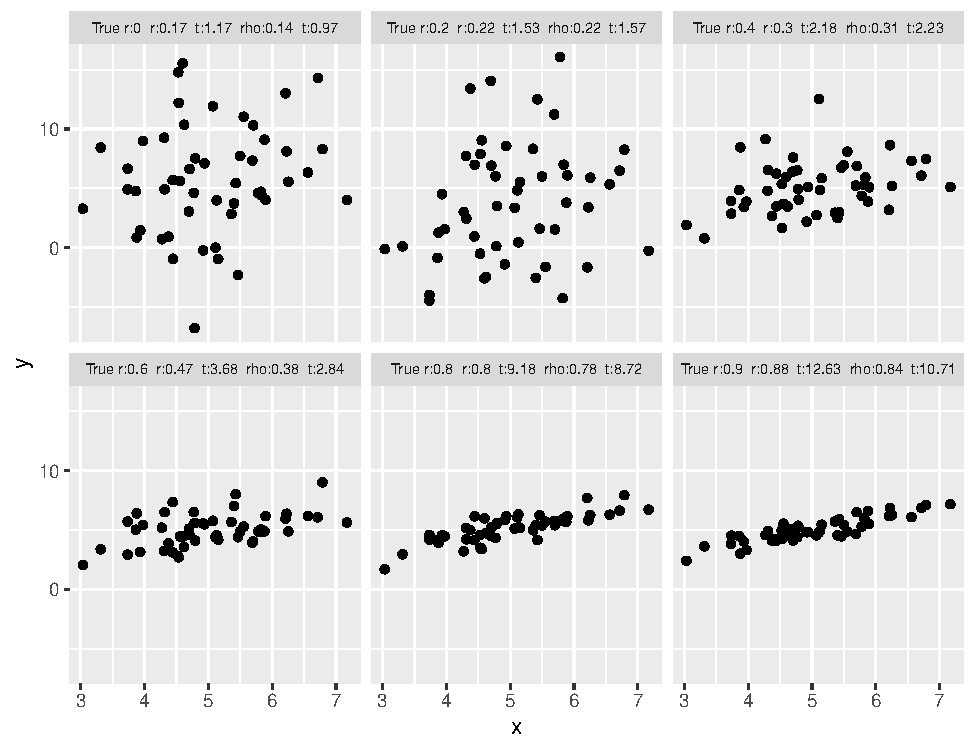
\includegraphics[width=\maxwidth]{corr-corrplota-1} }

\caption[Example correlation coefficients]{Samples of size $n=50$ for X and Y are drawn from bivariate normal populations with true correlations ranging from 0.0 to 0.9. Pearson and Spearman sample correlations are shown for samples of size 50.  Besides the population correlation coefficient, each panel is labeled with the estimated Pearson $r$, its $t$ statistic, the estimated Spearman $\rho$, and its $t$ statistic}\label{fig:corr-corrplota}
\end{figure}
\end{Schunk}
\begin{Schunk}
\begin{Sinput}
# Different scenarios that can lead to a correlation of 0.7

set.seed(123)   # Fig. (*\ref{fig:corr-corrplotb}*)
rho <- 0.7; n <- 50
var.eps <- rho^-2 - 1
x <- rnorm(n, 5, 1)
y <- x + rnorm(n, 0, sqrt(var.eps))
cor(x,y)
\end{Sinput}
\begin{Soutput}
[1] 0.6951673
\end{Soutput}
\begin{Sinput}
plot(x,y,xlab='',ylab='')

x <- c(1:20,30)
y <- c(1:20,6.2)
cor(x,y)
\end{Sinput}
\begin{Soutput}
[1] 0.6988119
\end{Soutput}
\begin{Sinput}
plot(x,y,xlab='',ylab='')

set.seed(123)
x <- rnorm(40)
y <- rnorm(40)
x[21] <- y[21] <- 8.5
cor(x,y)
\end{Sinput}
\begin{Soutput}
[1] 0.7014825
\end{Soutput}
\begin{Sinput}
plot(x,y,xlab='',ylab='')

x <- rep(0:19,2)
y <- c(rep(.62,20),rep(2,20)) * x
cor(x,y)
\end{Sinput}
\begin{Soutput}
[1] 0.701783
\end{Soutput}
\begin{Sinput}
plot(x,y,xlab='',ylab='')

x <- -7:12
y <- x^2
cor(x,y)
\end{Sinput}
\begin{Soutput}
[1] 0.6974104
\end{Soutput}
\begin{Sinput}
plot(x,y,xlab='',ylab='')

set.seed(123)
tmp <- 1:20 / 2
x <- c(rnorm(20, tmp, 1), tmp + rnorm(20,14.5,1))
y <- c(rnorm(20, -tmp, 1), -tmp + rnorm(20,14.5,1))
cor(x,y)
\end{Sinput}
\begin{Soutput}
[1] 0.703308
\end{Soutput}
\begin{Sinput}
plot(x,y,xlab='',ylab='')
\end{Sinput}
\begin{figure}[htbp]

\centerline{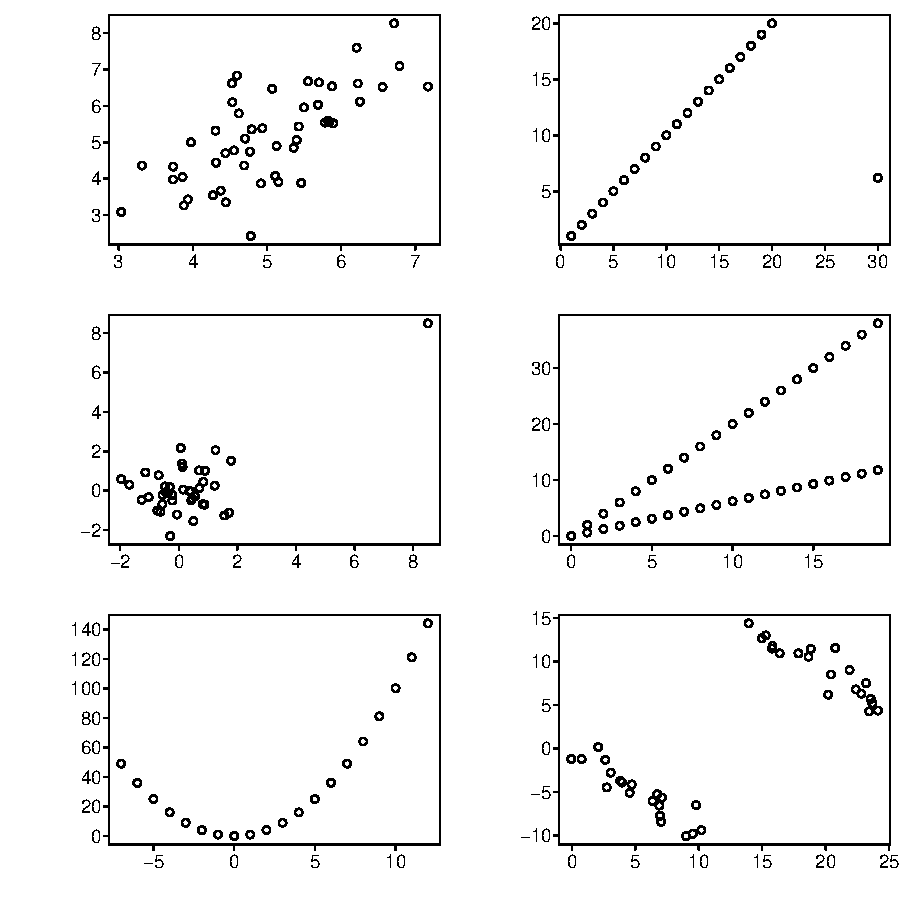
\includegraphics[width=\maxwidth]{corr-corrplotb-1} }

\caption[Multiple datasets having same Pearson $r$]{Different observed datasets that have the same correlation.  All six plots have a sample Pearson correlation of $0.7$.}\label{fig:corr-corrplotb}
\end{figure}
\end{Schunk}


\clearpage
\section{Correlation and Agreement}

\bi 
 \item Compare two methods of measuring the same underlying value
  \bi 
  \item Lung function measured using a spirometer (expensive, accurate) or peak flow meter (cheap, less accurate)
  \item Two devices (oropharyngeal and conventional) used to mesured
    acidity (pH) in the esophagus as a marker of reflux
  \ei
 \item Typical (incorrect) approach begins with scatterplot of one
   method vs.\ the other with a 1:1 line indicating perfect agreement
 \item See Figure~\ref{fig:descript-pH}
 \item Incorrect approach would report a high correlation ($r = 0.90$) and conclude good agreement
 \item Problems with the correlation approach
  \begin{enumerate}
   \item $r$ measures the degree of linear association between two
     variables, not the agreement.  If, for example, the Sandhill
     consistently gave pH values that were 0.5 unit higher than the
     Restech, we could still have high correlation, but poor agreement
     between the two devices.  We can have high correlation if the two
     devices lie closely to any line, not just a 1:1 line that
     indicates perfect agreement.  
   \item A change in scale does not affect correlation, but does
     influence agreement. For example, if the Sandhill always
     registered 2 times larger than the Restech, we would have perfect
     correlation but the agreement would get progressively worse for
     larger values of pH. 
   \item Correlation depends on the range of the data so that larger
     ranges lead to larger correlations.  This can lead to vary
     strange interpretations 

\begin{table}[!h]
\begin{center}
\begin{tabular}{l|cc}
 & $r$ & $\rho$ \\ \hline
all data & 0.90 & 0.73 \\ 
avg pH $\leq 4$ & 0.51 & 0.58 \\ 
avg pH $> 4$ & 0.74 & 0.65
\end{tabular}
\caption{Pearson ($r$) and Spearman ($\rho$) correlations for Restech and Sandhill pH data.  The correlation calculated using all of the data is larger than the correlation calculated using a retricted range of the data.  However, it would be difficult to claim that the overall agreement is better than both the agreement when pH is less than 4 and when pH is greater than 4.}
\end{center}
\end{table}

\item Tests of significance (testing if $r=0$) are irrelevant to the
  question at hand, but often reported to demonstrate a significant
  association.  The two devices are measuring the same quantity, so it
  would be shocking if we did not observe a highly significant
  $p$-value. A $p < .0001$ is not impressive.  A regression analysis
  with a highly significant slope would be similarly unimpressive. 
\item Data can have high correlation, but poor agreement.  There are
  many examples in the literature, but even in our analysis with $r =
  0.90$, the correlation is high, but we will show that the agreement
  is not as good as the high correlation implies. \
  \end{enumerate}
\ei

See Chapter~\ref{chap:obsvar} for simple approaches to assessing agreement
and analyzing observer variability studies.

\subsection{Bland-Altman Plots} \ems{36.4}

\bi 
  \item See Bland and Altman (1986, Lancet)
  \item Earlier: Tukey mean-difference plot
  \item Create plots of the difference in measurements on the y-axis
    versus the average value of the two devices on the x-axis 
  \item If the two devices agree, the difference should be about zero
  \item The average of the two devices is our best estimate of the
    true, unknown (pH) value that is we are trying to measure 
  \item Measurements will often vary in a systematic way over the
    range of measurement. By plotting the difference versus the
    average, we can visually determine if the difference changes over
    our estimate of the truth. 
  \item Solid line indicated the mean, dashed lines are approximate
    0.95 confidence intervals (assuming Normality) 
\ei

\textbf{But} there is controversy about what should be on the $x$-axis
of the plot.  Krouwer~\cite{kro08why} concluded that:
\bi
\item When the two measures have nearly equal variability, i.e., when
  comparing two ``field measurements'', the Bland-Altman approach is preferred
\item When one measurement is a ``reference standard'' having much less
  variation than the field measurement, the reference standard and not
  the average of the two measurements should be on the $x$-axis
\ei

\begin{Schunk}
\begin{Sinput}
require(Hmisc)
getHdata(esopH)
esopH$diff <- with(esopH, orophar - conv)
ggplot(esopH, aes(x=(conv + orophar)/2, y=diff)) +   # Fig. (*\ref{fig:corr-baplot}*)
  stat_binhex(aes(alpha=..count.., color=Hmisc::cut2(..count.., g=20)),
              bins=80) +
  stat_smooth() +
  geom_hline(yintercept = mean(esopH$diff, na.rm=TRUE) +
   c(-1.96, 0, 1.96) * sd(esopH$diff, na.rm=TRUE),
   linetype=c(2,1,2), color='brown') +
  xlab('Average of Conventional and Oropharyngeal pH') +
  ylab('Oropharyngeal Minus Conventional pH') +
  guides(alpha=FALSE, fill=FALSE, color=guide_legend(title='Frequency'))
\end{Sinput}
\begin{figure}[htbp]

\centerline{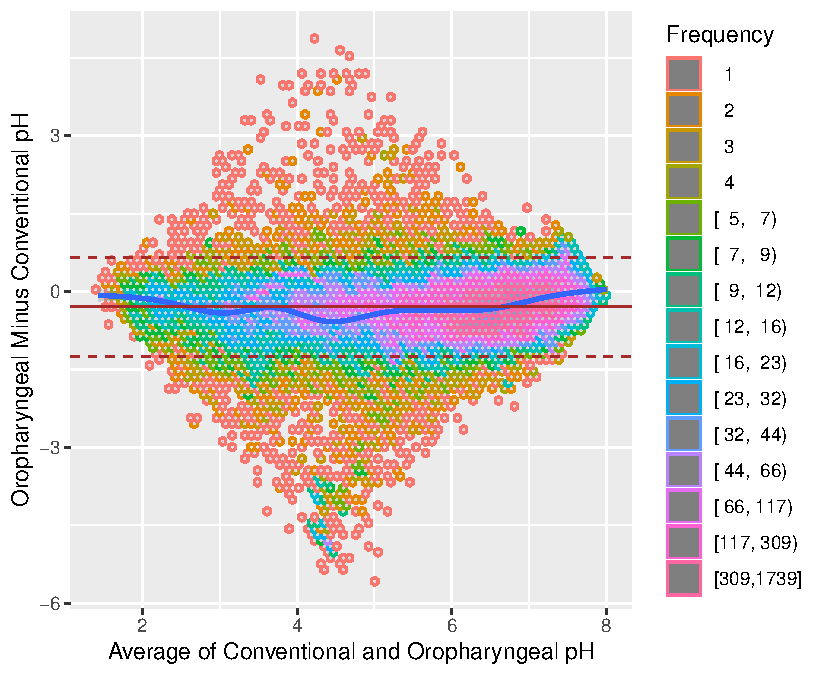
\includegraphics[width=\maxwidth]{corr-baplot-1} }

\caption[Bland-Altman plot for 2 pH measurements]{Bland-Altman plot for the oroesophageal and conventional pH measurements, using hexagonal binning because of the large sample size.  The difference in pH mesaurements (oro.\ -conventional) is presented on the $y$-axis and the average of the two devices on the $x$-axis.  We see poor agreement around pH values of 4-5}\label{fig:corr-baplot}
\end{figure}
\end{Schunk}

\bi 
  \item We will also consider differences in the two measurements over the time of day
  \item The added smooth curve is called a locally weighted scatterplot smooth (loess)
\ei

\begin{Schunk}
\begin{Sinput}
getHdata(esopH2)
ggplot(esopH2, aes(x=time, y=diffpH)) +    # Fig. (*\ref{fig:corr-phtimediff}*)
       geom_point(pch='.') + stat_smooth() +
       geom_hline(yintercept = 0, col='gray60') +
       scale_x_continuous(breaks=seq(16, 38, by=4),
                          labels=c("4 PM", "8 PM", "12 AM",
                            "4 AM", "8AM", "12 PM"),
                          limits=c(14, 14+24)) +
       ylab('Average of Oropharyngeal Minus Conventional pH') +
       xlab('Time of Day')
\end{Sinput}
\begin{figure}[htbp]

\centerline{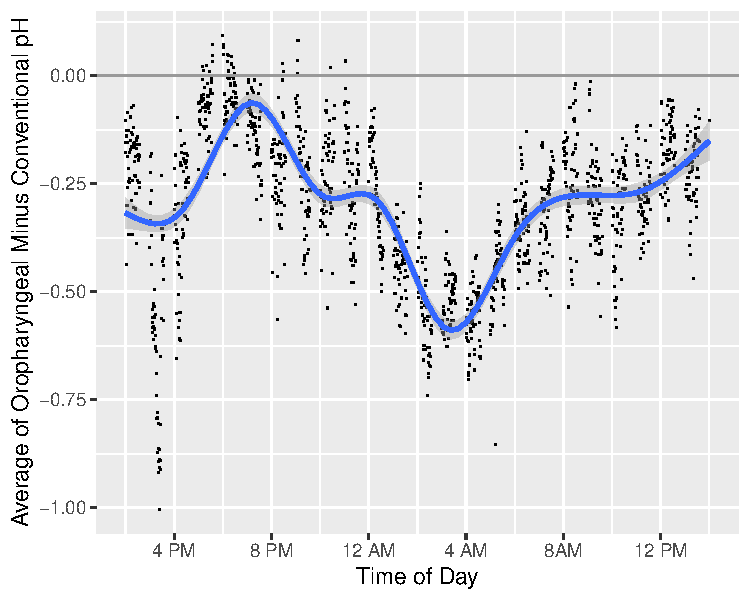
\includegraphics[width=\maxwidth]{corr-phtimediff-1} }

\caption[Difference in pH by time of day]{Difference in pH measurements (oro. - conventional) by time of day along with a loess smoother and pointwise 0.95 confidence bands.  Is the difference modified by a subject being in a supine position rather than being upright?}\label{fig:corr-phtimediff}
\end{figure}
\end{Schunk}

\subsection{Sample Size for $r$}\alabel{sec:corr-n}
\bi
\item Without knowledge of population variances, etc., $r$ can be
  useful for planning studies
\item Choose $n$ so that margin for error (half-width of C.L.) for $r$
  is acceptable
\item Precision of $r$ in estimating $\rho$ is generally worst when $\rho=0$
\item This margin for error as well as that for three other choices of the unknown true $\rho$ are shown in Figure~\ref{fig:corr-moe}.
\begin{Schunk}
\begin{Sinput}
require(Hmisc)
plotCorrPrecision(rho=c(0, .25, .5, .75),
                  n=seq(10, 1000, length=100),
                  ylim=c(0, .4), col=1:4, opts=list(keys='lines'))
abline(h=seq(0, .4, by=0.025),
       v=seq(25, 975, by=25), col=gray(.9))
\end{Sinput}
\begin{figure}[htbp]

\centerline{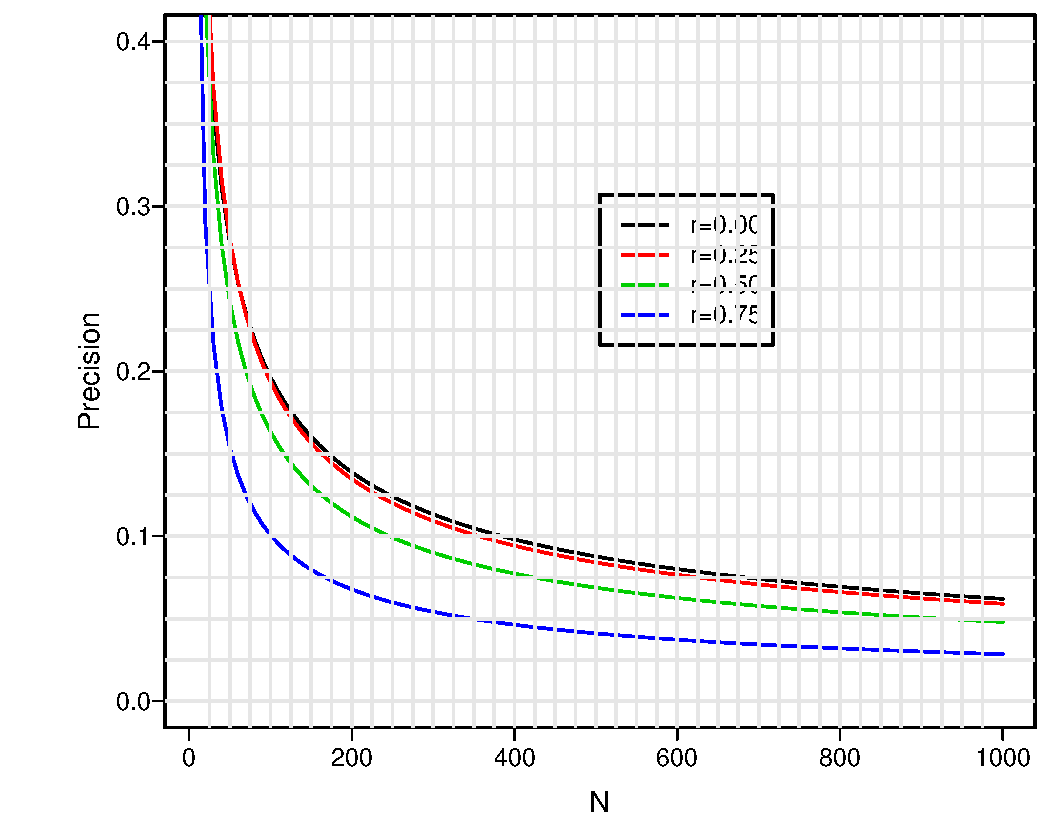
\includegraphics[width=\maxwidth]{corr-moe-1} }

\caption[Margin of error for estimating correlation coefficient]{Margin for error (length of longer side of asymmetric 0.95 confidence interval) for $r$ in estimating $\rho$, when $\rho=0, 0.25, 0.5, 0.75$.  Calculations are based on Fisher $z$ transformation of $r$.}\label{fig:corr-moe}
\end{figure}
\end{Schunk}
\ei

See also \href{https://stats.stackexchange.com/questions/415131}{stats.stackexchange.com/questions/415131}.

\subsection{Comparing Two $r$'s}
\bi
\item Rarely appropriate
\item Two $r$'s can be the same even though slopes may differ
\item Usually better to compare effects on a real scale (slopes)
\ei
